%\documentclass[table]{beamer}
%[]中可以使用draft、handout、screen、transparency、trancompress、compress等参数

%指定beamer的模式与主题
\mode<presentation>
{
  \usetheme{Madrid}
%\usetheme{Boadilla}
%\usecolortheme{default}
%\usecolortheme{orchid}
%\usecolortheme{whale}
%\usefonttheme{professionalfonts}
}

%\usetheme{Madrid}
%这里还可以选择别的主题:Bergen, Boadilla, Madrid, AnnArbor, CambridgeUS, Pittsburgh, Rochester, Warsaw, ...
%有导航栏的Antibes, JuanLesPins, Montpellier, ...
%有内容的Berkeley, PaloAlto, Goettingen, Marburg, Hannover, ...
%有最小导航栏的Berlin, Ilmenau, Dresden, Darmstadt, Frankfurt, Singapore, Szeged, ...
%有章和节表单的Copenhagen, Luebeck, Malmoe, Warsaw, ...

%\usecolortheme{default}
%设置内部颜色主题(这些主题一般改变block里的颜色);这个主题一般选择动物来命名
%这里还可以选择别的颜色主题,如默认的和有特别目的的颜色主题default,structure,sidebartab,全颜色主题albatross,beetle,crane,dove,fly,seagull,wolverine,beaver

%\usecolortheme{orchid}
%设置外部颜色主题(这些主题一般改变title里的颜色);这个主题一般选择植物来命名
%这里还可以选择别的颜色主题,如默认的和有特别目的的颜色主题lily,orchid,rose

%\usecolortheme{whale}
%设置字体主题;这个主题一般选择海洋动物来命名
%这里还可以选择别的颜色主题,如默认的和有特别目的的颜色主题whale,seahorse,dolphin

%\usefonttheme{professionalfonts}
%类似的还可以定义structurebold,structuresmallcapsserif,professionalfonts


% 控制 beamer 的风格,可以根据自己的爱好修改
%\usepackage{beamerthemesplit} %使用 split 风格
%\usepackage{beamerthemeshadow} %使用 shadow 风格
%\usepackage[width=2cm,dark,tab]{beamerthemesidebar}


% 设定英文字体
%\usepackage{fontspec}
\usepackage[no-math]{fontspec}
\setmainfont{Times New Roman}
\setsansfont{Arial}
\setmonofont{Courier New}

% 设定中文字体
\usepackage[BoldFont,SlantFont,CJKchecksingle,CJKnumber]{xeCJK}
%\setCJKmainfont[BoldFont={Adobe Heiti Std},ItalicFont={Adobe Kaiti Std}]{Adobe Song Std}
\setCJKmainfont[BoldFont={Adobe Heiti Std},ItalicFont={Adobe Kaiti Std}]{WenQuanYi Micro Hei}
\setCJKsansfont{Adobe Heiti Std}
\setCJKmonofont{Adobe Fangsong Std}
\punctstyle{hangmobanjiao}

\defaultfontfeatures{Mapping=tex-text}
\usepackage{xunicode}
\usepackage{xltxtra}

\XeTeXlinebreaklocale "zh"
\XeTeXlinebreakskip = 0pt plus 1pt minus 0.1pt

\usepackage{setspace}
\usepackage{colortbl,xcolor}
\usepackage{hyperref}
%\hypersetup{xetex,bookmarksnumbered=true,bookmarksopen=true,pdfborder=1,breaklinks,colorlinks,linkcolor=blue,filecolor=black,urlcolor=cyan,citecolor=green}
\hypersetup{xetex,bookmarksnumbered=true,bookmarksopen=true,pdfborder=1,breaklinks,colorlinks,linkcolor=cyan,filecolor=black,urlcolor=blue,citecolor=green}

% 插入图片
\usepackage{graphicx}
\graphicspath{{figures/}}

% 可能用到的包
\usepackage{amsmath,amssymb}
\usepackage{multimedia}
\usepackage{multicol}
\usepackage{multirow}

% 定义一些自选的模板,包括背景、图标、导航条和页脚等,修改要慎重
% 设置背景渐变由10%的红变成10%的结构颜色
%\beamertemplateshadingbackground{red!10}{structure!10}
%\beamertemplatesolidbackgroundcolor{white!90!blue}
% 使所有隐藏的文本完全透明、动态,而且动态的范围很小
\beamertemplatetransparentcovereddynamic
% 使itemize环境中变成小球,这是一种视觉效果
\beamertemplateballitem
% 为所有已编号的部分设置一个章节目录,并且编号显示成小球
\beamertemplatenumberedballsectiontoc
% 将每一页的要素的要素名设成加粗字体
\beamertemplateboldpartpage

% item逐步显示时,使已经出现的item、正在显示的item、将要出现的item呈现不同颜色
\def\hilite<#1>{
 \temporal<#1>{\color{gray}}{\color{blue}}
    {\color{blue!25}}
}

\renewcommand{\today}{\number\year 年 \number\month 月 \number\day 日}

%五角星
\usepackage{MnSymbol}

%去除图表标题中的figure等
\usepackage{caption}
\captionsetup{labelformat=empty,labelsep=none}

\usepackage{tabu}
\usepackage{multirow}

% 千分号
%\usepackage{textcomp}

%罗马数字
\makeatletter
\newcommand{\rmnum}[1]{\romannumeral #1}
\newcommand{\Rmnum}[1]{\expandafter\@slowromancap\romannumeral #1@}
\makeatother

%分栏
\usepackage{multicol}

%\usepackage{enumitem}
\usepackage{enumerate}


%\setbeamercolor{alerted text}{fg=magenta}

\setbeamercolor{bgcolor}{fg=yellow,bg=cyan}

\begin{document}

%\includeonlyframes{current}

\logo{\includegraphics[height=0.08\textwidth]{tijmu.png}}
\title[基因组功能注释分析]{基因组功能注释分析}
\author[Yixf]{伊现富(Yi Xianfu)}
\institute[TIJMU]{天津医科大学(TIJMU)\\ 生物医学工程学院}
\date{2013年9月}


% 在每个Section前都会加入的Frame
\AtBeginSection[]
{
  \begin{frame}<beamer>
    %\frametitle{Outline}
    \frametitle{教学提纲}
	\setcounter{tocdepth}{2}
	\begin{multicols}{2}
    %\tableofcontents[currentsection,currentsubsection]
    \tableofcontents[currentsection]
	\end{multicols}
  \end{frame}
}
% 在每个Subsection前都会加入的Frame
%\AtBeginSubsection[]
%{
  %\begin{frame}<beamer>
%%\begin{frame}<handout:0>
%% handout:0 表示只在手稿中出现
    %\frametitle{Outline}
	%\setcounter{tocdepth}{2}
    %\tableofcontents[currentsection,currentsubsection]
%% 显示在目录中加亮的当前章节
  %\end{frame}
%}

\begin{frame}[plain]
	\begin{center}
		{\Huge 生物信息学\\}
		\vspace{1cm}
		{\LARGE 天津医科大学\\}
		%\vspace{0.2cm}
		{\LARGE 生物医学工程学院\\}
		\vspace{1cm}
		{\large 2013-2014学年上学期}
	\end{center}
\end{frame}

\begin{frame}
  \titlepage
\end{frame}

\begin{frame}[plain]
  \frametitle{教学提纲}
  \setcounter{tocdepth}{2}
  \begin{multicols}{2}
  \tableofcontents
  \end{multicols}
\end{frame}

\section{引言}
\begin{frame}
	\frametitle{基因组注释}
	\begin{block}{基因组注释(genome annotation)}
		\begin{itemize}
			\item 结构注释(structural annotation)
			\item 功能注释(functional annotation)
		\end{itemize}
	\end{block}
\end{frame}

\begin{frame}
	\frametitle{引言 | NGS}
	\begin{center}
		\includegraphics[width=10cm]{ngs.jpg}
	\end{center}
\end{frame}

\section{基因组组装版本}
\begin{frame}
	\frametitle{基因组组装版本 | XP VS. Win7}
	\begin{center}
		\includegraphics[width=9cm]{windows.jpg}
	\end{center}
\end{frame}

\begin{frame}
	\frametitle{基因组组装版本 | 版本对照}
	\begin{table}
		\centering
		\rowcolors[]{1}{blue!20}{blue!10}
		\begin{tabular}{cccc}
			\hline
			\rowcolor{blue!50} SPECIES & UCSC & DATE & NCBI\\
			Human & hg19 & Feb. 2009 & Genome Reference Consortium\\
			 & & & GRCh37\\
			 & hg18 & Mar. 2006 & NCBI Build 36.1\\
			 & hg17 & May 2004 & NCBI Build 35\\
			 & hg16 & Jul. 2003 & NCBI Build 34\\
			 & hg15 & Apr. 2003 & NCBI Build 33\\
			\hline
			Mouse & mm10 & Dec. 2011 & Genome Reference Consortium\\
			 & & & GRCm38\\
			 & mm9 & Jul. 2007 & NCBI Build 37\\
			 & mm8 & Feb. 2006 & NCBI Build 36\\
			 & mm7 & Aug. 2005 & NCBI Build 35\\
			 & mm6 & Mar. 2005 & NCBI Build 34\\
			\hline
		\end{tabular}
	\end{table}
\end{frame}

\section{基因组坐标系统}
\begin{frame}
	\frametitle{坐标系统 | 坐标轴}
	\begin{center}
		\includegraphics[width=6cm]{2d.png}
	\end{center}
	\visible<2->{
	\begin{center}
		\includegraphics[width=8cm]{1d.jpg}
	\end{center}
	}
\end{frame}

\begin{frame}
	\frametitle{坐标系统}
	\begin{block}{序列}
	\begin{table}
		\centering
		\rowcolors[]{1}{blue!20}{blue!10}
		\begin{tabular}{lcccccccc}
			\hline
			0-based index & 0 & 1 & 2 & 3 & 4 & 5 & 6 & 7\\
			\hline
			Sequence & A & A & T & T & G & G & C & C\\
			\hline
			1-based index & 1 & 2 & 3 & 4 & 5 & 6 & 7 & 8\\
			\hline
		\end{tabular}
	\end{table}
	\end{block}
	\pause
	\begin{block}{TG的坐标}
		\begin{itemize}
			\item 0-based,half-open:[3,5)
			\item 1-based,fully-closed:[4,5]
		\end{itemize}
	\end{block}
	\pause
	\begin{block}{实例}
		\begin{itemize}
			\item 0-based:BED、BAM、PSL,dbSNP、Table Browser
			\item 1-based:GFF、VCF、SAM、Wiggle,DAS、Genome Browser
		\end{itemize}
	\end{block}
\end{frame}

\begin{frame}
	\frametitle{坐标系统 | 类比}
	\begin{columns}
	\column{0.5\textwidth}
	\visible<1->{
	\begin{block}{first floor}
		\begin{center}
			\includegraphics[width=6cm]{firstFloor.jpg}
		\end{center}
	\end{block}
	}
	\column{0.48\textwidth}
	\visible<2->{
	\begin{block}{数组}
		\begin{center}
			\includegraphics[width=5.5cm]{array.png}
		\end{center}
	\end{block}
	}
	\end{columns}
\end{frame}

\section{基因组注释常用格式}
\begin{frame}
	\frametitle{格式 | FASTA}
		\begin{center}
			\includegraphics[width=12cm]{fasta.png}
		\end{center}
\end{frame}

\begin{frame}
	\frametitle{格式 | IUB/IUPAC核酸}
		\begin{center}
			\includegraphics[width=8cm]{iub.png}
		\end{center}
\end{frame}

\begin{frame}
	\frametitle{格式 | IUB/IUPAC氨基酸}
		\begin{center}
			\includegraphics[width=11cm]{aa.png}
		\end{center}
\end{frame}

\begin{frame}
	\frametitle{格式 | BED}
		\begin{center}
			\includegraphics[width=12cm]{bed.png}
		\end{center}
\end{frame}

\begin{frame}
	\frametitle{格式 | GFF}
		\begin{center}
			\includegraphics[width=12cm]{gff.png}
		\end{center}
\end{frame}

\begin{frame}
	\frametitle{格式 | VCF}
		\begin{center}
			\includegraphics[width=12cm]{vcf.png}
		\end{center}
\end{frame}

\begin{frame}
	\frametitle{格式 | 文本编辑器}
		\begin{center}
			\includegraphics[width=9cm]{editor.png}
		\end{center}
\end{frame}

\section{基因组坐标的逻辑运算模式}
\begin{frame}
	\frametitle{逻辑运算 | 集合运算}
		\begin{center}
			\includegraphics[width=9cm]{set.png}
		\end{center}
\end{frame}

\begin{frame}
	\frametitle{逻辑运算 | 集合 $\Rightarrow$ 基因组}
		\begin{center}
			\includegraphics[width=9cm]{setT.png}
		\end{center}
\end{frame}

%\begin{frame}
	%\frametitle{逻辑运算 | 运算模式}
		%\begin{center}
			%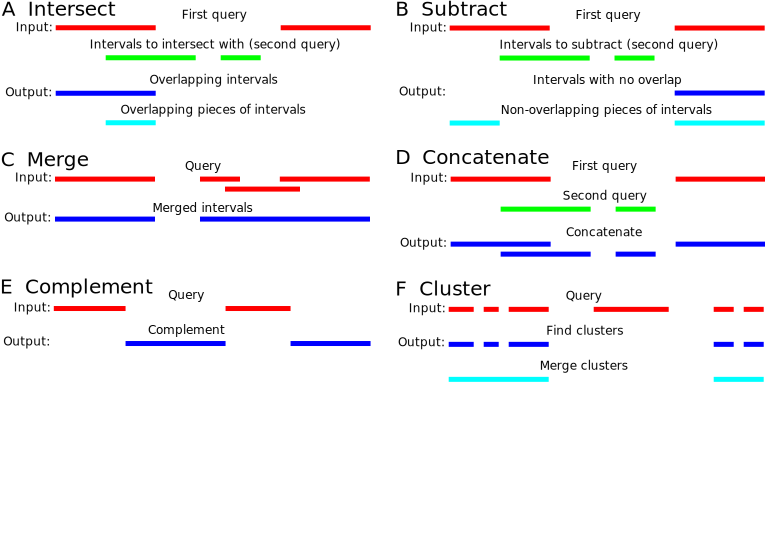
\includegraphics[width=12cm]{operation.png}
		%\end{center}
%\end{frame}

\begin{frame}
	\frametitle{逻辑运算 | intersect}
		\begin{center}
			\includegraphics[width=10cm]{intersect.png}
			\vspace{0.1cm}
			%\includegraphics[width=9cm]{intersectA.png}\\
			\includegraphics[width=10cm]{intersectB.png}
		\end{center}
\end{frame}

\begin{frame}
	\frametitle{逻辑运算 | subtract}
		\begin{center}
			\includegraphics[width=10cm]{subtract.png}
			\vspace{0.1cm}
			\includegraphics[width=10cm]{subtractB.png}
		\end{center}
\end{frame}

\begin{frame}
	\frametitle{逻辑运算 | merge}
		\begin{center}
			\includegraphics[width=10cm]{merge.png}
			\vspace{0.5cm}
			\includegraphics[width=10cm]{mergeB.png}
		\end{center}
\end{frame}

\begin{frame}
	\frametitle{逻辑运算 | concatenate}
		\begin{center}
			\includegraphics[width=10cm]{concat.png}
		\end{center}
\end{frame}

\begin{frame}
	\frametitle{逻辑运算 | complement}
		\begin{center}
			\includegraphics[width=10cm]{complement.png}
			\vspace{0.1cm}
			\includegraphics[width=10cm]{complementA.png}
			\vspace{0.1cm}
			\includegraphics[width=10cm]{complementB.png}
		\end{center}
\end{frame}

\begin{frame}
	\frametitle{逻辑运算 | cluster}
		\begin{center}
			\includegraphics[width=10cm]{cluster.png}
			\vspace{0.1cm}
			\includegraphics[width=10cm]{clusterB.png}
		\end{center}
\end{frame}

\begin{frame}
	\frametitle{逻辑运算 | join}
		\begin{center}
			\includegraphics[width=11cm]{join.png}
		\end{center}
\end{frame}

\section{操作演示}
\begin{frame}
	\frametitle{操作演示 | liftOver}
	\begin{enumerate}[<+-|alert@+>]
		\item 获取输入
			\begin{itemize}
				\item 输入文件:hg19坐标
			\end{itemize}
		\item 数据处理
			\begin{itemize}
				\item 设置参数:hg19 $\Rightarrow$ hg18
			\end{itemize}
		\item 保存输出
			\begin{itemize}
				\item 过滤结果:MAPPED VS. UNMAPPED
			\end{itemize}
	\end{enumerate}
\end{frame}

\begin{frame}
	\frametitle{操作演示 | BED $\Leftrightarrow$ GFF}
	\begin{enumerate}[<+-|alert@+>]
		\item 获取输入
			\begin{itemize}
				\item 输入文件:BED
			\end{itemize}
		\item 数据处理
			\begin{enumerate}
				\item BED $\Rightarrow$ GFF
				\item GFF $\Rightarrow$ BED
			\end{enumerate}
		\item 保存输出
			\begin{itemize}
				\item 查看结果:互相比较
			\end{itemize}
	\end{enumerate}
\end{frame}

\begin{frame}
	\frametitle{操作演示| subtract \& join}
	\begin{enumerate}[<+-|alert@+>]
		\item 获取输入
			\begin{itemize}
				\item exon
				\item SNP
			\end{itemize}
		\item 数据处理
			\begin{itemize}
				\item subtract
				\item join
			\end{itemize}
		\item 保存输出
			\begin{itemize}
				\item 解析结果
			\end{itemize}
	\end{enumerate}
\end{frame}

\section{总结与答疑}
\begin{frame}
	\frametitle{总结与答疑}
	\begin{block}{知识点}
		\begin{itemize}
			\item 基因组组装版本的对应关系
			\item 两种坐标系统——0-based和1-based
			\item 四种常用格式——FASTA,BED,GFF,VCF
			\item 坐标的逻辑运算模式
			\item 坐标转换、格式转换、逻辑运算的工具
		\end{itemize}
	\end{block}
	\begin{block}{技能}
		\begin{itemize}
			\item “输入-加工-输出”三段论
			\item 获取输入
			\item 数据处理
			\item 解析输出
		\end{itemize}
	\end{block}
\end{frame}

\section{引言}
\begin{frame}
	\frametitle{引言}
	\begin{block}{前期准备工作}
		\begin{itemize}
			\item 组装版本
			\item 坐标转换
			\item 常用格式
			\item 逻辑运算
		\end{itemize}
	\end{block}
	\pause
	\begin{block}{后续功能注释}
		\begin{itemize}
			\item 变异位点的注释
			\item 基因集富集分析
			\item 制作序列标识
		\end{itemize}
	\end{block}
	\pause
	\begin{block}{分析平台}
		\begin{itemize}
			\item Galaxy
		\end{itemize}
	\end{block}
\end{frame}

\section{变异位点的注释}
\begin{frame}
	\frametitle{变异位点的注释 | 注释工具}
	\begin{itemize}
		\item SeattleSeq Annotation、variant tools、SnpEff 
		\item SIFT、PolyPhen-2、SNPs3D
		\item PROVEAN
	\end{itemize}
\end{frame}

\begin{frame}
	\frametitle{变异位点的注释 | 结果解析 | SeattleSeq Annotation}
		\begin{center}
			\includegraphics[width=12cm]{seattleseqannotation.png}
		\end{center}
\end{frame}

\begin{frame}
	\frametitle{变异位点的注释 | 结果解析 | SIFT}
		\begin{center}
			\includegraphics[width=12cm]{siftannotation.png}
		\end{center}
\end{frame}

\section{基因集富集分析}
\begin{frame}
	\frametitle{富集分析 | 数据库与分析工具}
	\begin{itemize}
		\item GO
		\item KEGG
		\item DAVID
	\end{itemize}
\end{frame}

\begin{frame}
	\frametitle{富集分析 | DAVID}
	\begin{itemize}
		\item Gene Name Batch Viewer
		\item Gene ID Conversion Tool
		\item Gene Functional Classification Tool
		\item Functional Annotation Tool
		\begin{itemize}
			\item Functional Annotation Clustering
			\item Functional Annotation Chart:富集分析
			\item Functional Annotation Table
		\end{itemize}
	\end{itemize}
\end{frame}

\begin{frame}
	\frametitle{富集分析 | DAVID | 结果解析}
	\begin{center}
		\includegraphics[width=9cm]{david.png}
	\end{center}
\end{frame}

\begin{frame}
	\frametitle{富集分析 | DAVID | 工具选择}
	\begin{center}
		\includegraphics[width=10cm]{david2.png}
	\end{center}
\end{frame}

\section{序列标识}
\begin{frame}
	\frametitle{序列标识}
	\begin{block}{序列标识(sequence logo)}
		\begin{itemize}
			\item 横轴:位置
			\item 纵轴:比特
			\item 总高度:保守性
			\item 相对高度:相对频率
			\item 制作工具:WebLogo, enoLOGOS
		\end{itemize}
	\end{block}
\end{frame}

\begin{frame}
	\frametitle{序列标识 | 剪接}
	\begin{center}
		\includegraphics[width=12cm]{gtag.png}\\
	\end{center}
\end{frame}

\begin{frame}
	\frametitle{序列标识 | 实例}
	\begin{center}
		\includegraphics[width=10cm]{donor.png}\\
		\includegraphics[width=10cm]{acceptor.png}
	\end{center}
\end{frame}

\begin{frame}
	\frametitle{序列标识 | 实例 | 真实数据}
	\begin{table}
		\centering
		\rowcolors[]{1}{blue!20}{blue!10}
		\begin{tabular}{cc|cc}
			\hline
			\rowcolor{blue!50} \multicolumn{2}{c|}{Donor Sites(\%)} & \multicolumn{2}{c}{Acceptor Site(\%)}\\
			\hline
			GT & 98.797 & AG & 99.714\\
			GC & 0.920 & AC & 0.120\\
			AT & 0.143 & TG & 0.032\\
			GA & 0.028 & AT & 0.024\\
			GG & 0.025 & GG & 0.022\\
			CT & 0.018 & AA & 0.019\\
			TT & 0.016 & CG & 0.010\\
			CC & 0.011 & CC & 0.010\\
			TG & 0.007 & TT & 0.009\\
			AG & 0.007 & CT & 0.008\\
			TA & 0.006 & CA & 0.008\\
			AC & 0.006 & GC & 0.007\\
			CA & 0.006 & TA & 0.006\\
			TC & 0.004 & TC & 0.004\\
			AA & 0.004 & GT & 0.004\\
			CG & 0.002 & GA & 0.003\\
			\hline
		\end{tabular}
	\end{table}
\end{frame}

\section{Galaxy分析平台}
\begin{frame}
	\frametitle{Galaxy | 工具集}
	\begin{itemize}
		\item Get Data
		\item Text Manipulation
		\item Convert Formats
		\item Operate on Genomic Intervals
		\item Phenotype Association
		\item Statistics
		\item Graph/Display Data
		\item NGS Toolbox
		\item \ldots
	\end{itemize}
\end{frame}

\begin{frame}
	\frametitle{Galaxy | 界面}
	\begin{center}
		\includegraphics[width=12cm]{galaxy.png}
	\end{center}
\end{frame}

\section{Galaxy操作实例}
\begin{frame}
	\frametitle{Galaxy | 实例}
	\begin{block}{Finding exons with the highest number of SNPs}
	\begin{enumerate}[<+-|alert@+>]
		\item Input: exons, snps; UCSC Table Browser
		\item Join[Genomic Operations Join]: identify those exons that contain SNPs
		\item Group: obtain the number of SNPs within each exon
		\item Sort: sort exon by SNP count
		\item Filter: filter exons that have ten or more SNPs
		\item Join[Join two Queries]: restore genomic location for exons containing ten or more SNPs
		\item Visualize: visualize dataset in UCSC Genome Browser
	\end{enumerate}
	\end{block}
\end{frame}


\section{总结与答疑}
\begin{frame}
	\frametitle{总结与答疑}
	\begin{block}{知识点}
		\begin{itemize}
			\item 变异位点注释的用途及注释工具
			\item 基因集富集分析的功能及分析工具
			\item 序列标识的含义与制作工具
			\item Galaxy分析平台的使用方法
		\end{itemize}
	\end{block}
	\begin{block}{技能}
		\begin{itemize}
			\item 查找工具使用的protocol
			\item 学习新工具的方法与步骤
			\item 数据处理流程的保存与共享
		\end{itemize}
	\end{block}
\end{frame}

\section*{Acknowledgements}
\begin{frame}
	\frametitle{Powered by}
	\begin{center}
		\includegraphics[width=9cm]{power.png}
	\end{center}
\end{frame}

\end{document}
